\ifdefined\ishandout
\documentclass[handout, 10pt]{beamer}
\else
\documentclass[10pt]{beamer}
\fi

%\usepackage[frenchb]{babel}
\usepackage[T1]{fontenc}
%\usepackage[utf8]{inputenc}
\usepackage{hyperref}
\usepackage{multirow}
\usepackage{listings}
\usepackage{fancyvrb}
\usepackage{tikz}
\usepackage{framed}
\usepackage{xmpmulti}
\usepackage{algorithm}
\usepackage{algorithmicx}
\usepackage{algpseudocode}
\usepackage{xcolor}
\usepackage{booktabs}
\usepackage{color, colortbl}
\ifdefined\ishandout
\usepackage{handoutWithNotes}
\fi
\usepackage{slashbox}
\usepackage{amsmath}
\usepackage{bm}
\usepackage{hhline}
\usepackage{pgfplots}
\usepackage{caption}
\graphicspath{{../old/course-utrecht/fig/}{../old/course-utrecht/fig/L1/}{../old/course-utrecht/fig/L2/}{../old/course-utrecht/fig/L3/}} %Setting the graphicspath

\def\UrlBreaks{\do\/\do-}

\usetikzlibrary{shapes.geometric}
\usetikzlibrary{positioning}
\usetikzlibrary{shapes.arrows, chains}
\usetikzlibrary{arrows,calc}
\usetikzlibrary{shapes.multipart}
\usetikzlibrary{matrix}

\usepackage{array}
%\usetheme{Boadilla}
\usetheme[progressbar=frametitle]{metropolis}

\usefonttheme[onlymath]{serif}

\newcommand{\R}{\mathbb{R}}
%\newcommand{\C}{\mathbb{C}}
\newcommand{\N}{\mathbb{N}}
\newcommand{\Z}{\mathbb{Z}}
\newcommand{\E}{\mathbb{E}}
\newcommand{\Var}{\text{Var}}
\newcommand{\Cov}{\text{Cov}}
\ifdefined\ishandout
\pgfpagesuselayout{3 on 1 with notes}[a4paper,border shrink=5mm]
\usecolortheme{dove}
\else
%\usecolortheme{dolphin}
%\usecolortheme{crane}
\fi

\metroset{block=fill}

\lstnewenvironment{codeC}
{ \lstset{language=C,
    otherkeywords={printf,scanf}}
}
{}

\ifdefined\ishandout
\definecolor{mygreen}{rgb}{0,0,0}
\definecolor{mymauve}{rgb}{0,0,0}
\definecolor{myblue}{rgb}{0,0,0}
\else
\definecolor{mygreen}{rgb}{0,0.6,0}
\definecolor{mymauve}{rgb}{0.58,0,0.82}
\definecolor{myblue}{rgb}{0,0,1}

\fi

%% Notes
%\setbeameroption{show only notes}


\definecolor{mygray}{rgb}{0.5,0.5,0.5}

\lstset{ language=Python,%
  backgroundcolor=\color{white},   % choose the background color; you must add \usepackage{color} or \usepackage{xcolor}
  basicstyle=\footnotesize,        % the size of the fonts that are used for the code
  breakatwhitespace=false,         % sets if automatic breaks should only happen at whitespace
  breaklines=true,                 % sets automatic line breaking
  captionpos=b,                    % sets the caption-position to bottom
  commentstyle=\color{mygreen},    % comment style
  deletekeywords={...},            % if you want to delete keywords from the given language
  escapeinside={\%*}{*)},          % if you want to add LaTeX within your code
  extendedchars=true,              % lets you use non-ASCII characters; for 8-bits encodings only, does not work with UTF-8
  frame=tb,	                   % adds a frame around the code
  keepspaces=true,                 % keeps spaces in text, useful for keeping indentation of code (possibly needs columns=flexible)
  keywordstyle=\color{blue},       % keyword style
  otherkeywords={*,...},           % if you want to add more keywords to the set
  numbers=none,                    % where to put the line-numbers; possible values are (none, left, right)
  numbersep=5pt,                   % how far the line-numbers are from the code
  numberstyle=\tiny\color{mygray}, % the style that is used for the line-numbers
  rulecolor=\color{black},         % if not set, the frame-color may be changed on line-breaks within not-black text (e.g. comments (green here))
  showspaces=false,                % show spaces everywhere adding particular underscores; it overrides 'showstringspaces'
  showstringspaces=false,          % underline spaces within strings only
  showtabs=false,                  % show tabs within strings adding particular underscores
  stepnumber=2,                    % the step between two line-numbers. If it's 1, each line will be numbered
  stringstyle=\color{mymauve},     % string literal style
  tabsize=3,	                   % sets default tabsize to 2 spaces
  title=\lstname                   % show the filename of files included with \lstinputlisting; also try caption instead of title
}
%\lstset{language=Python,
% breakatwhitespace=false,         % sets if automatic breaks should only happen at whitespace
%  breaklines=true,                 % sets automatic line breaking
%  captionpos=b,                
%%commentstyle=\itshape\color{mymauve},
%%keywordstyle=\bfseries\color{myblue},
%numbers=left,                    % where to put the line-numbers; possible values are (none, left, right)
%  numbersep=8pt,                   % how far the line-numbers are from the code
%  numberstyle=\tiny\color{mygray}, % the style that is used for the line-numbers
%%  rulecolor=\color{black},         % if not set, the frame-color may be changed on line-breaks within not-black text (e.g. comments (green here))
%  showspaces=false,                % show spaces everywhere adding particular underscores; it overrides 'showstringspaces'
%%  showstringspaces=false,          % underline spaces within strings only
%  showtabs=false,                  % show tabs within strings adding particular underscores
%  stepnumber=2,                    % the step between two line-numbers. If it's 1, each line will be numbered
%%  stringstyle=\color{mygreen},     % string literal style
%  tabsize=2 
%}
\ifdefined\ishandout
\newcommand{\red}{\textbf}
\else
\newcommand{\red}{\textcolor{red}}
\fi
%\newcommand \emph
%Default size : 12.8 cm * 9.6 cm

\newcommand{\tmark}[1]{\tikz[remember picture, baseline=-.5ex]{\coordinate(#1);}}

\definecolor{bluegreen}{RGB}{0,149,182}


%\newcommand{\output}[1]{
\setbeamertemplate{navigation symbols}{}
\newcommand{\bvrb}{\Verb[commandchars=£µ§,formatcom=\color{bluegreen}]}
\newcommand{\footvrb}{\footnotesize\Verb}
\newcommand{\vrbalert}[2][]{\visible<#1>{#2}}
%%% Commande pour les listes/arbres
\newcommand{\mvide}{\nodepart{one} \nodepart{two}}
\newcommand{\tvide}{\nodepart{one} \nodepart{two} \nodepart{three}}
\newcommand{\rref}[1][]{\hfill{\scriptsize\textit{#1}}}

%%Fin des commandes pour les listes/arbres.



%%% Paramètres du cours (à régler)
%Numéro du cours
\newcommand{\nb}{1}

\title[Machine Learning]{Machine learning and physical (Earth system) modelling - course 1}
\author[J. Brajard]{julien.brajard@nersc.no}
\institute[NERSC]{NERSC\\
slides+notebook:\url{https://github.com/nansencenter/nersc_ml_course}}
\date{October 2021}

\begin{document}
%%%%%%%%%%%%%%%%%%%%% SLIDES DE TITRE
\begin{frame}
\titlepage
\end{frame}



%%%%%%%%%%%%%%%%%%%%%
\begin{frame}{References}
    \bibliographystyle{alpha}
    \nocite{Goodfellow-et-al-2016,VanderPlas-2016}
\bibliography{myref.bib}
\end{frame}

\begin{frame}[allowframebreaks]{Table of contents}
  \setbeamertemplate{section in toc}[sections numbered]
  \tableofcontents[hideallsubsections]
\end{frame}




\section{Introduction}

%%%%%%%%%%%%%%%%%%%%%
\begin{frame}{Scope of the lecture: Machine Learning}
%\centering
%  \begin{tikzpicture}[scale=0.9]
%    \draw<3-> {(0,0) ellipse (2 and 1)};
%    \draw<2-> {(0.3,0.3) ellipse (2.5 and 1.5)};
%    \draw<1-> {(0.6,0.6) ellipse (3.1 and 2.1)};
%    \draw<5->[line width = 0.5mm]  {(0.3,0.3) ellipse (2.5 and 1.5)};
%     \node<3-> at (0,0) {Deep Learning};
 % \node<2-> at (.3,1.2) {\alert<5->{Machine Learning}};
 % \node<1-> at (0.7,2) {Artificial intelligence};
 % \end{tikzpicture}  
 \begin{center}
     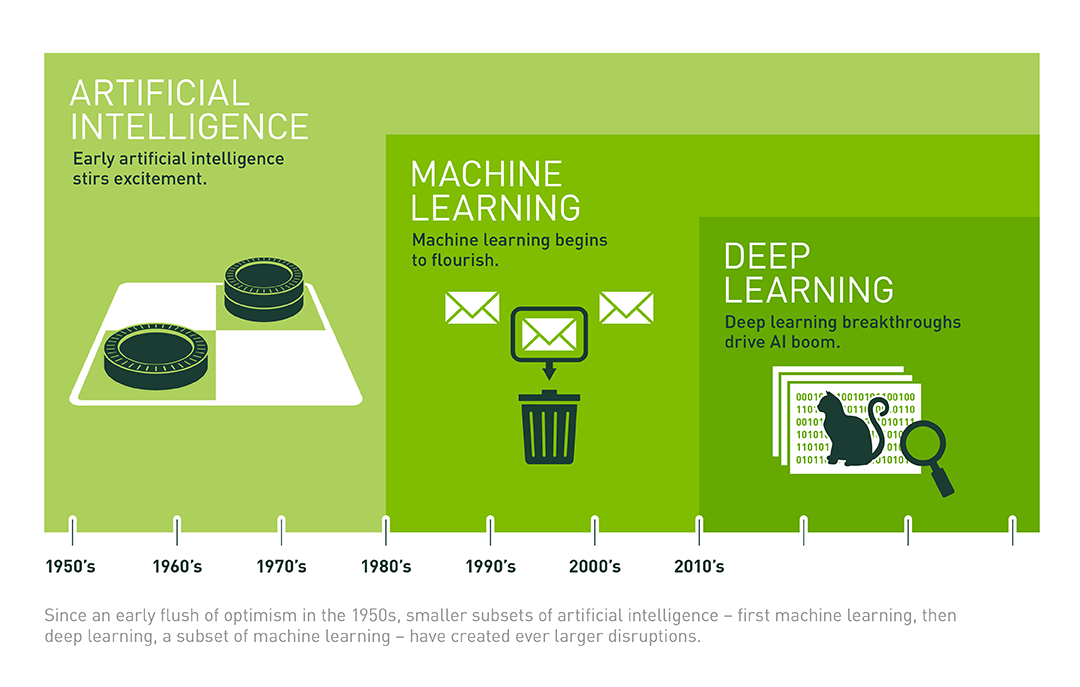
\includegraphics[width=\textwidth]{Deep_Learning_Icons_R5_PNG.png}
 \end{center}
 \rref[Source: NVidia]
 \end{frame}
 \begin{frame}{A (very) active field}

\begin{figure}
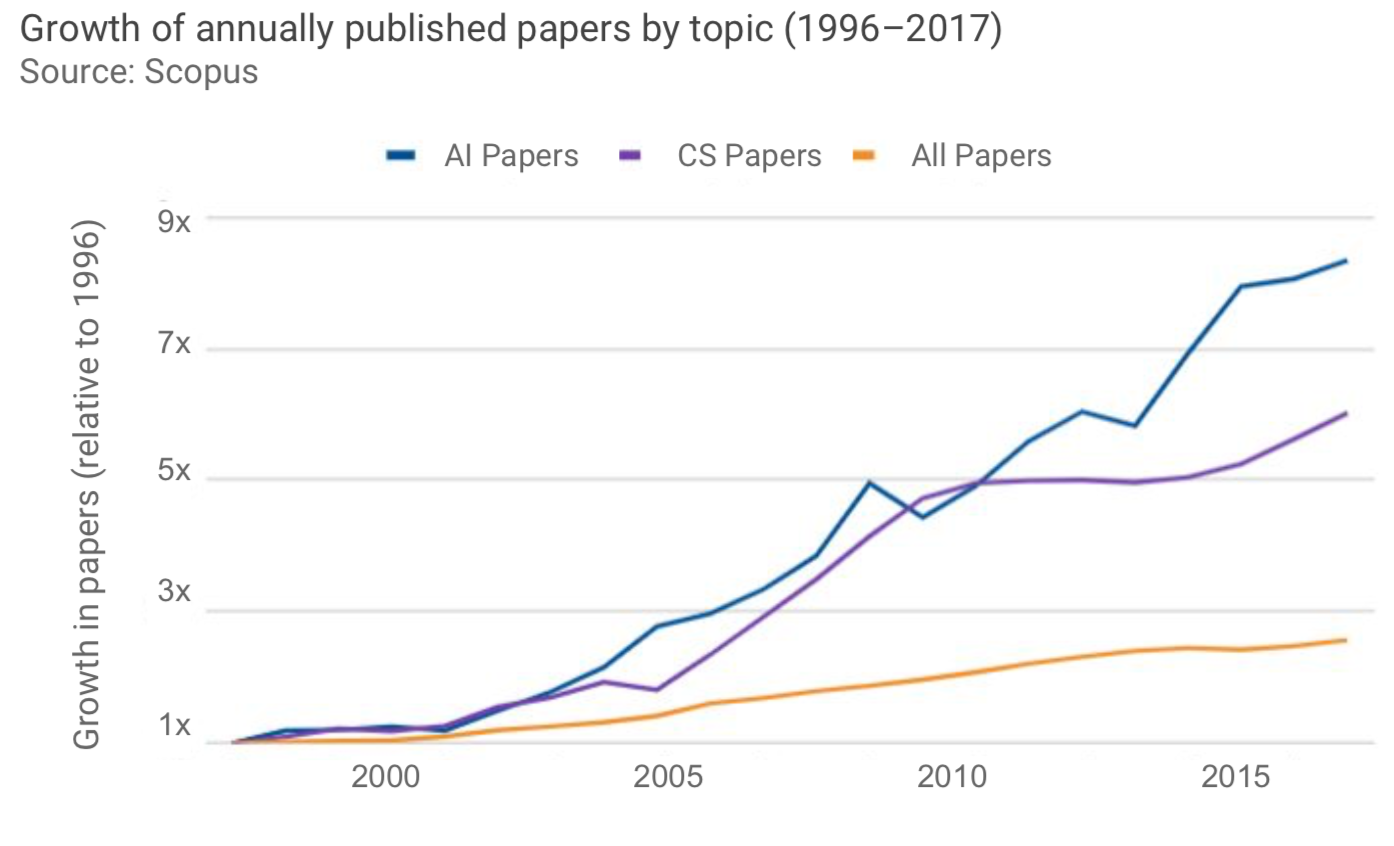
\includegraphics[width=.6\textwidth]{/progress-papers.png}
\end{figure}

\begin{figure}
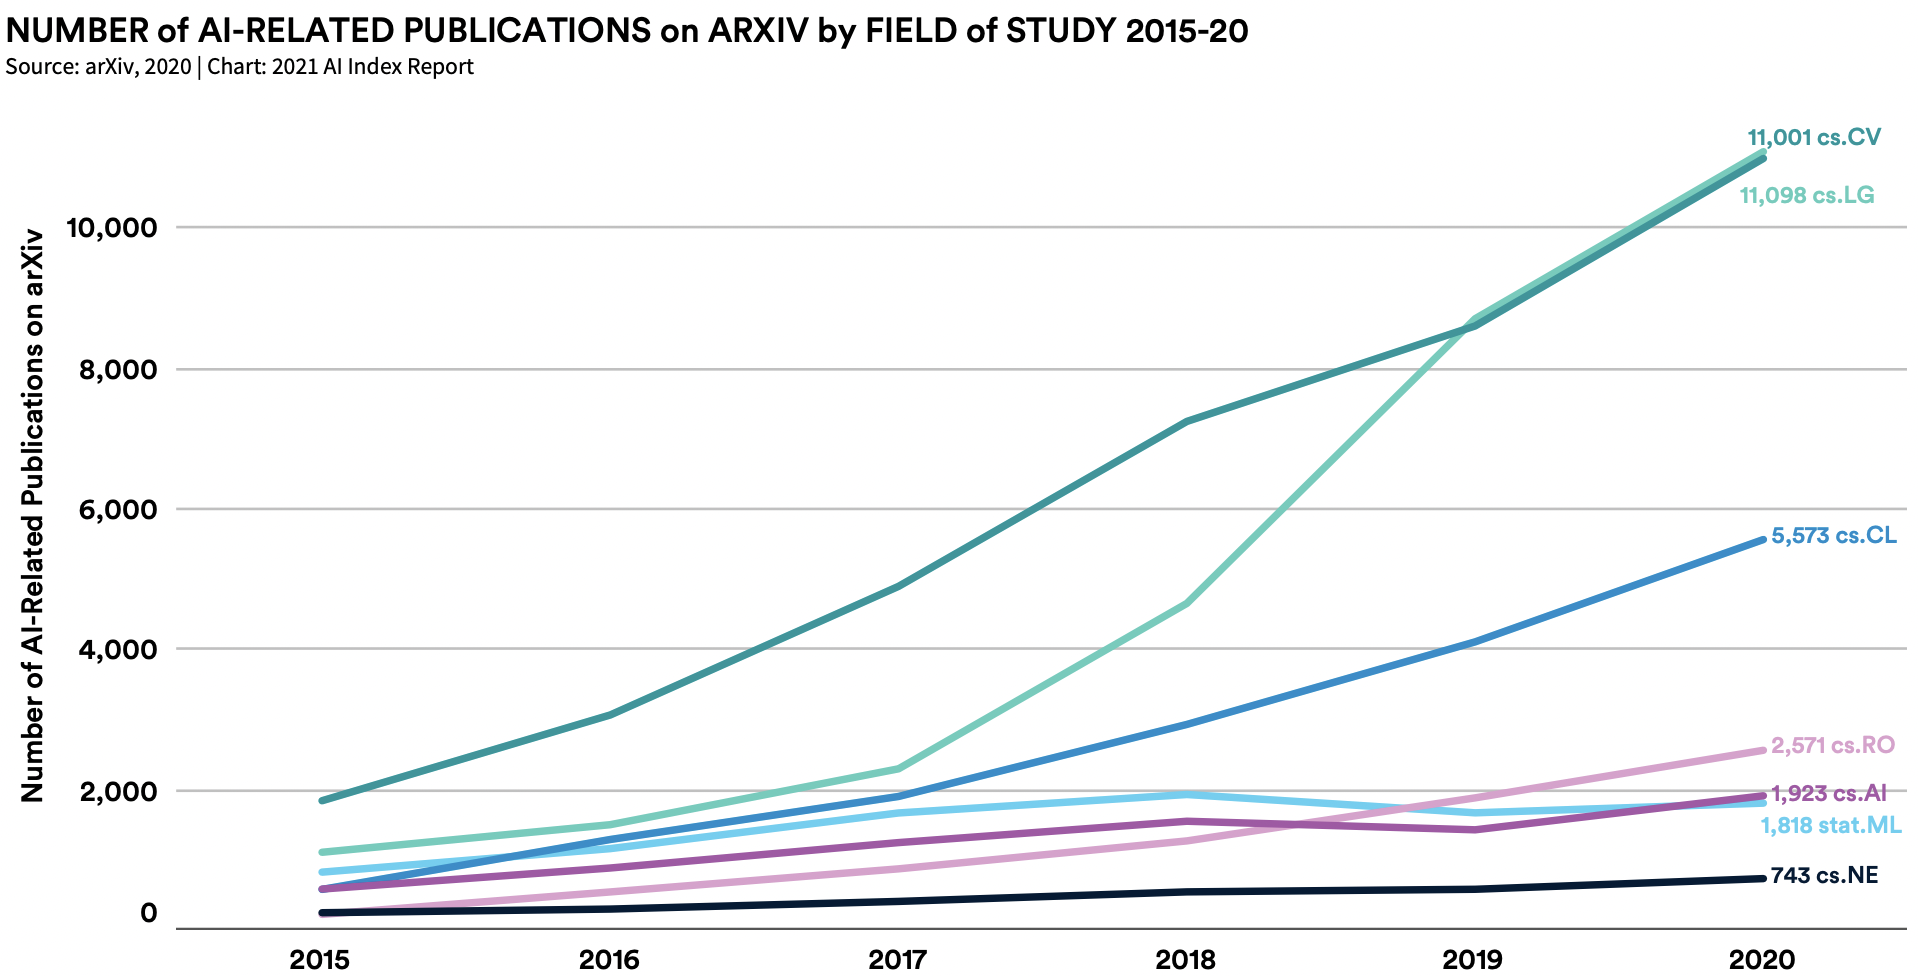
\includegraphics[width=.6\textwidth]{progress-ml.png}
\end{figure}

  \rref[Zhang et al., ``The AI Index 2021 Annual Report´´]

\end{frame}



%%%%%%%%%%%%%%%%%%%%
\begin{frame}
\frametitle{Example 1: Computer Vision}
\begin{figure}
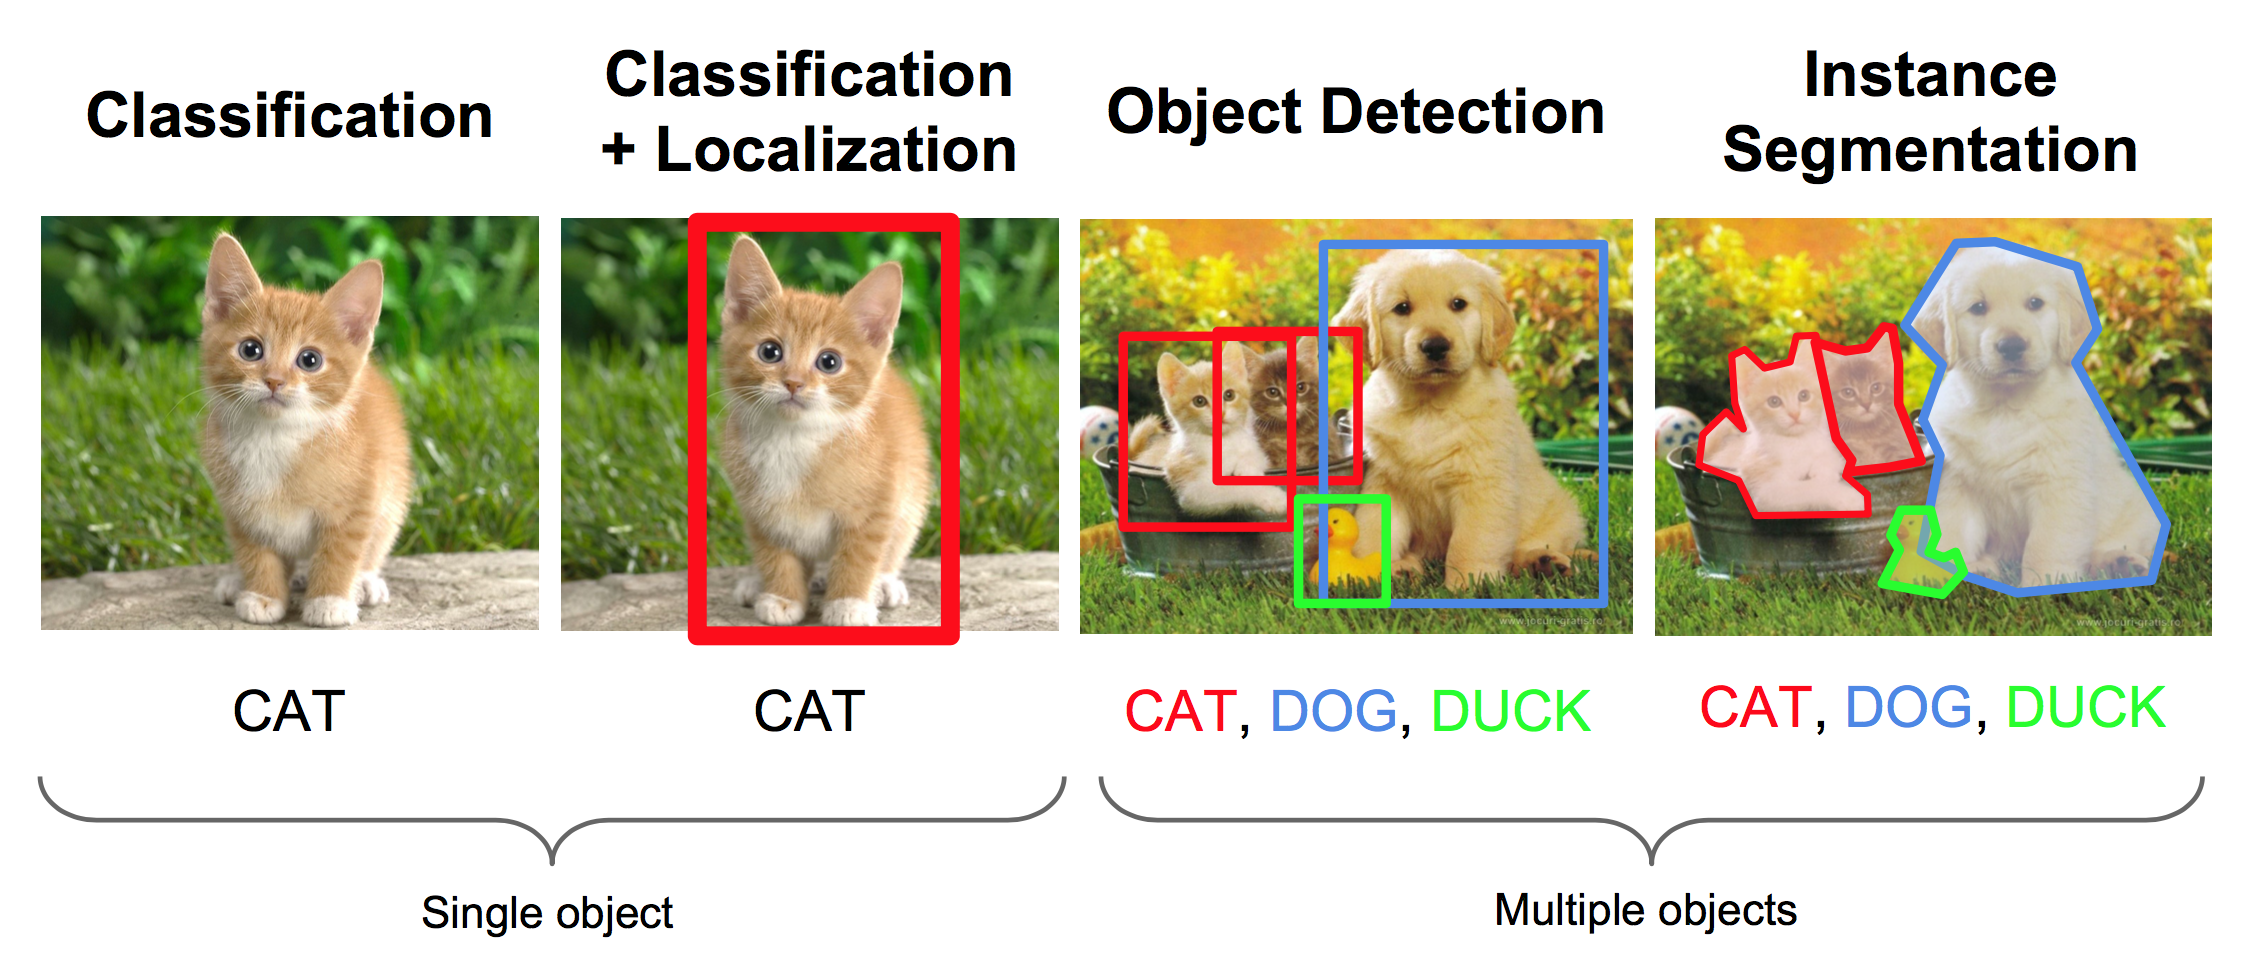
\includegraphics[width=\textwidth]{compute-vision.png}
\end{figure}
\rref[Li, Karpathy and Johnson, 2016, Stanford CS231n course]

\end{frame}


%%%%%%%%%%%%%%%%%%%%
\begin{frame}
\frametitle{Example 1: Computer Vision}
\framesubtitle{Image Net Large Scale Recogonition Challenge (ILSVRC)}
\begin{figure}

\begin{tikzpicture} [scale=0.8, every node/.style={scale=0.6}]
  \begin{axis}[ 
    x tick label style={ 
      /pgf/number format/1000 sep=}, 
    ylabel=Classification error, 
    xtick={2010,2011,2012,2013,2014,2015,2016,2017},
    xticklabels={2010,2011,2012,2013,2014,2015,2016,hum.},
    enlargelimits=0.15, 
     bar width=7pt, 
    ybar,
   legend style={at={(0.5,-0.15)},
     anchor=north,legend columns=-1}, 
   x tick label style={font=\footnotesize,rotate=45, anchor=east},
   very axis plot/.append style={
      ybar,
      bar width=.2,
      bar shift=0pt,
      fill},
      nodes near coords,
   ] 
   \addplot[ybar,fill=blue!60, bar shift=0pt]
   coordinates {(2010,28) (2011,26)}; 
   \addplot[ybar,fill=red!60]
   coordinates {(2012,16) (2013,12) (2014,7) (2015,3.6) (2016,3)}; 
   \addplot[ybar,fill=green!60, bar shift=0pt] 
   coordinates 
   {(2017,5.1)};  
   \legend{traditional algo.,Deep Learning,Human}
 \end{axis} 
\end{tikzpicture}
\end{figure}
Deep learning architectures were based on Convolutional Neural Networks (CNN).
\end{frame}



%%%%%%%%%%%%%%%%%%%%
\begin{frame}
\frametitle{Example 2: Machine Translation}
Objective : translate a text from a language to another.
\begin{figure}
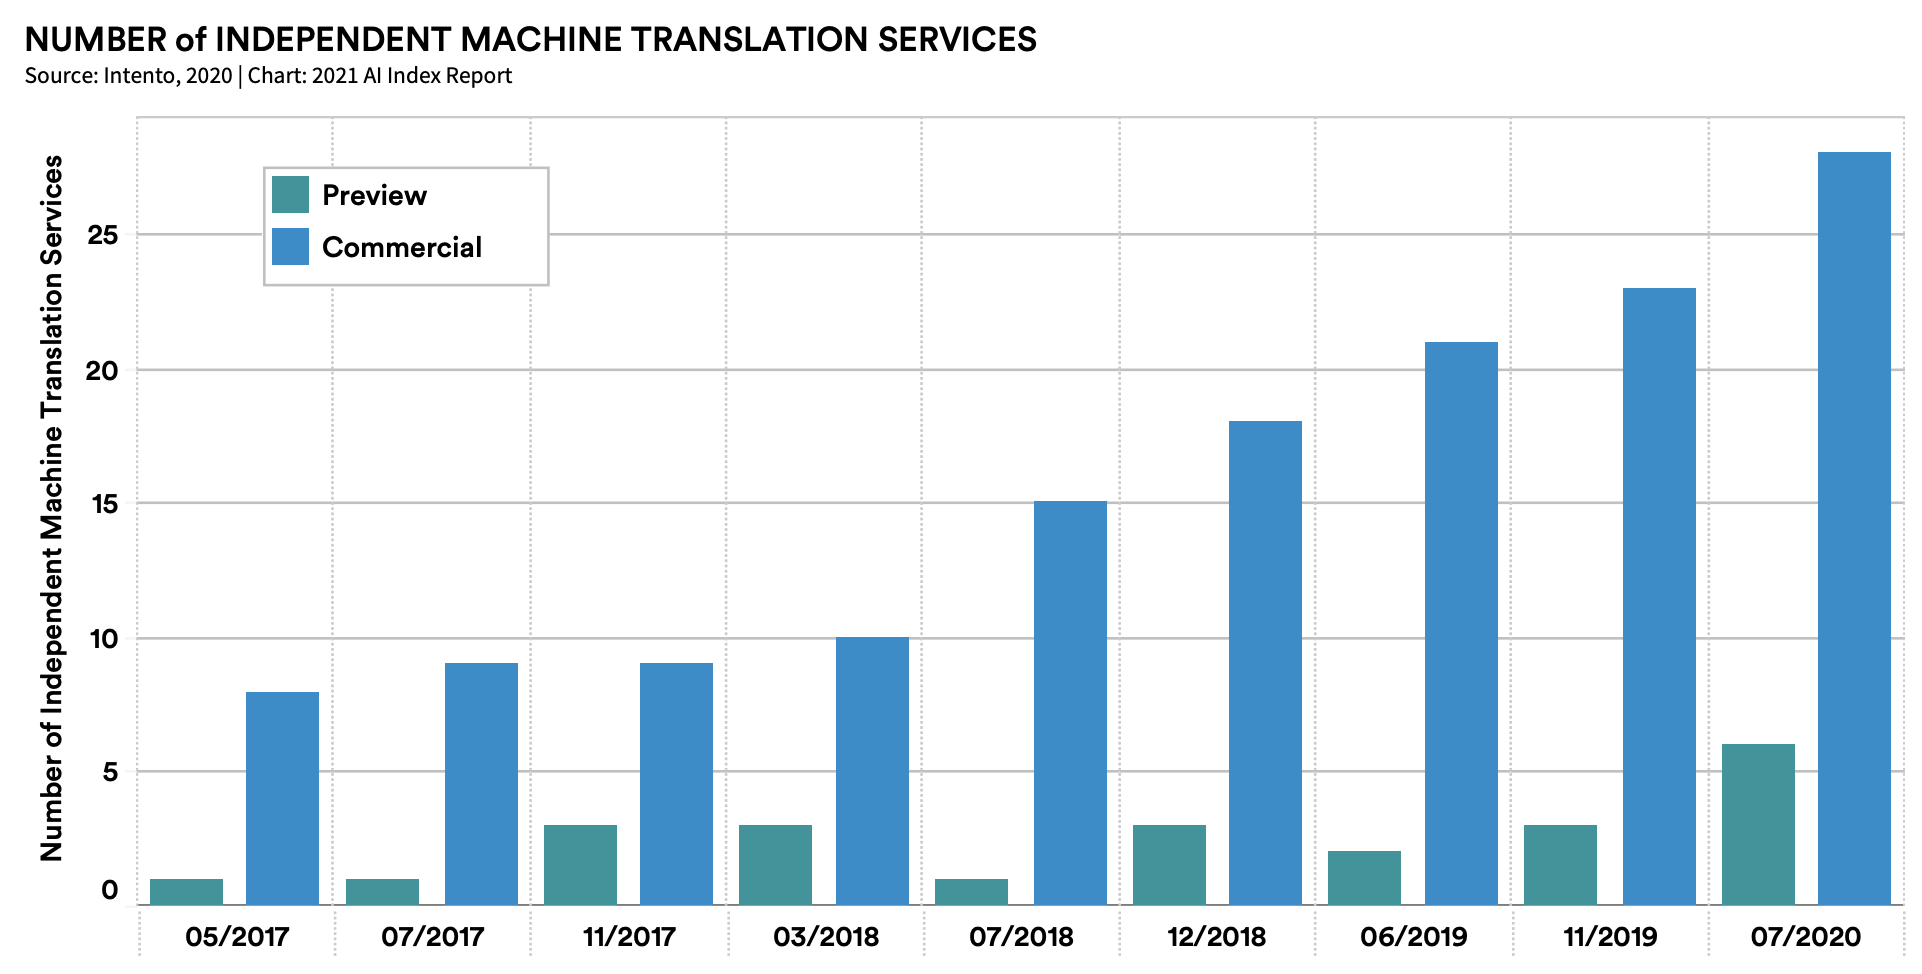
\includegraphics[width=.5\textwidth]{progress-machine-translation.png}\\
  \rref[Zhang et al., ``The AI Index 2021 Annual Report´´]

\end{figure}

\begin{itemize}
\item {\bf Oct. 2013}: Pionneering scientic paper  (Kalchbrenner, N., and Blunsom, P).
\item {\bf 2016}: Neural machine translation outperform traditional approaches on public benchmarks
\item {\bf 2017}: Major systems  switch to
  neural machine translation  (using deep recurrent neural networks)
\end{itemize}
\end{frame}



%%%%%%%%%%%%%%%%%%%%
\begin{frame}
\frametitle{Example 3: Playing Games}
\begin{columns}
\column{.5\textwidth}
\begin{itemize}
\item {\bf 1997}: Deep Blue defeats Kasparov at Chess.
\item {\bf 2016}: AlphaGo's victory again Lee Sedol at Go.
\item {\bf 2017}: AphaGo Zero learns how to play Go only by playing against
  itself. It outperformed previous AlphaGo version (Reinforcement
  learning)
\item {\bf 2017}: DeepStack beats professional human poker players.
\end{itemize}
\column{.5\textwidth}
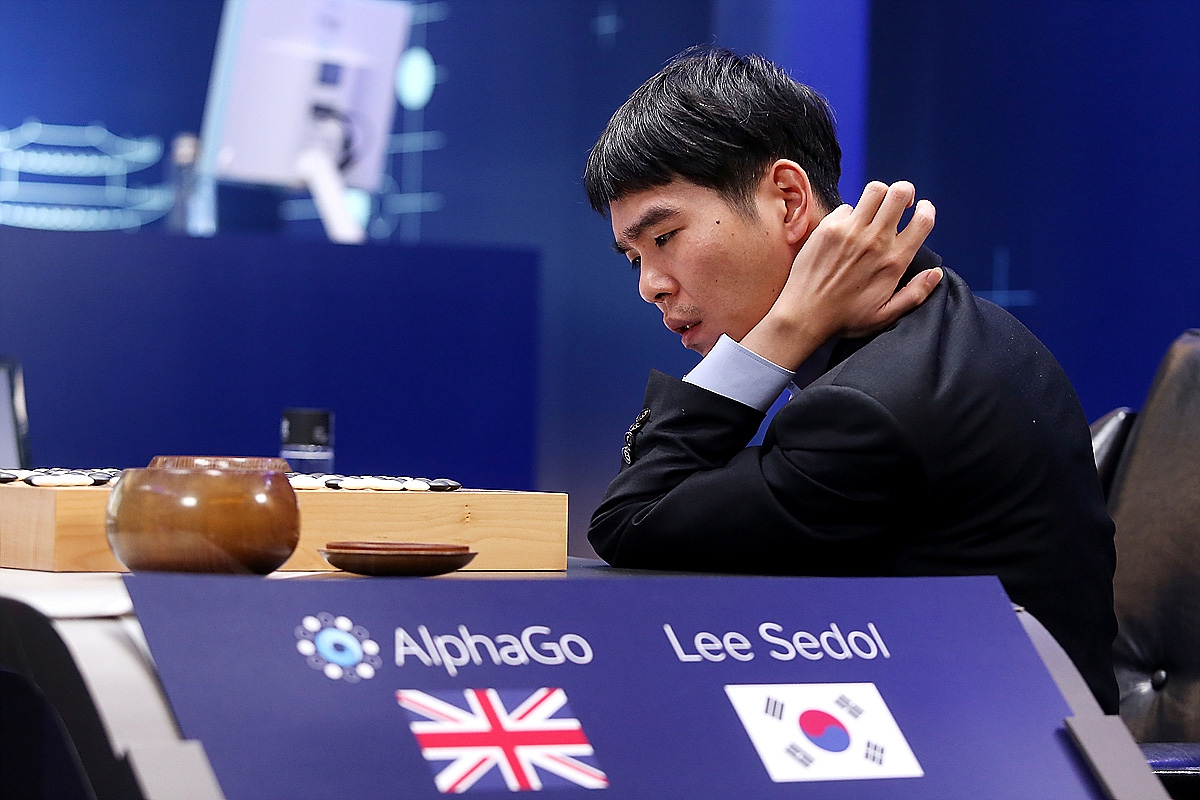
\includegraphics[width=\textwidth]{alphago.jpg}
\end{columns}
\end{frame}

\begin{frame}{Example 4: Protein folding}
  \begin{figure}
        \centering
        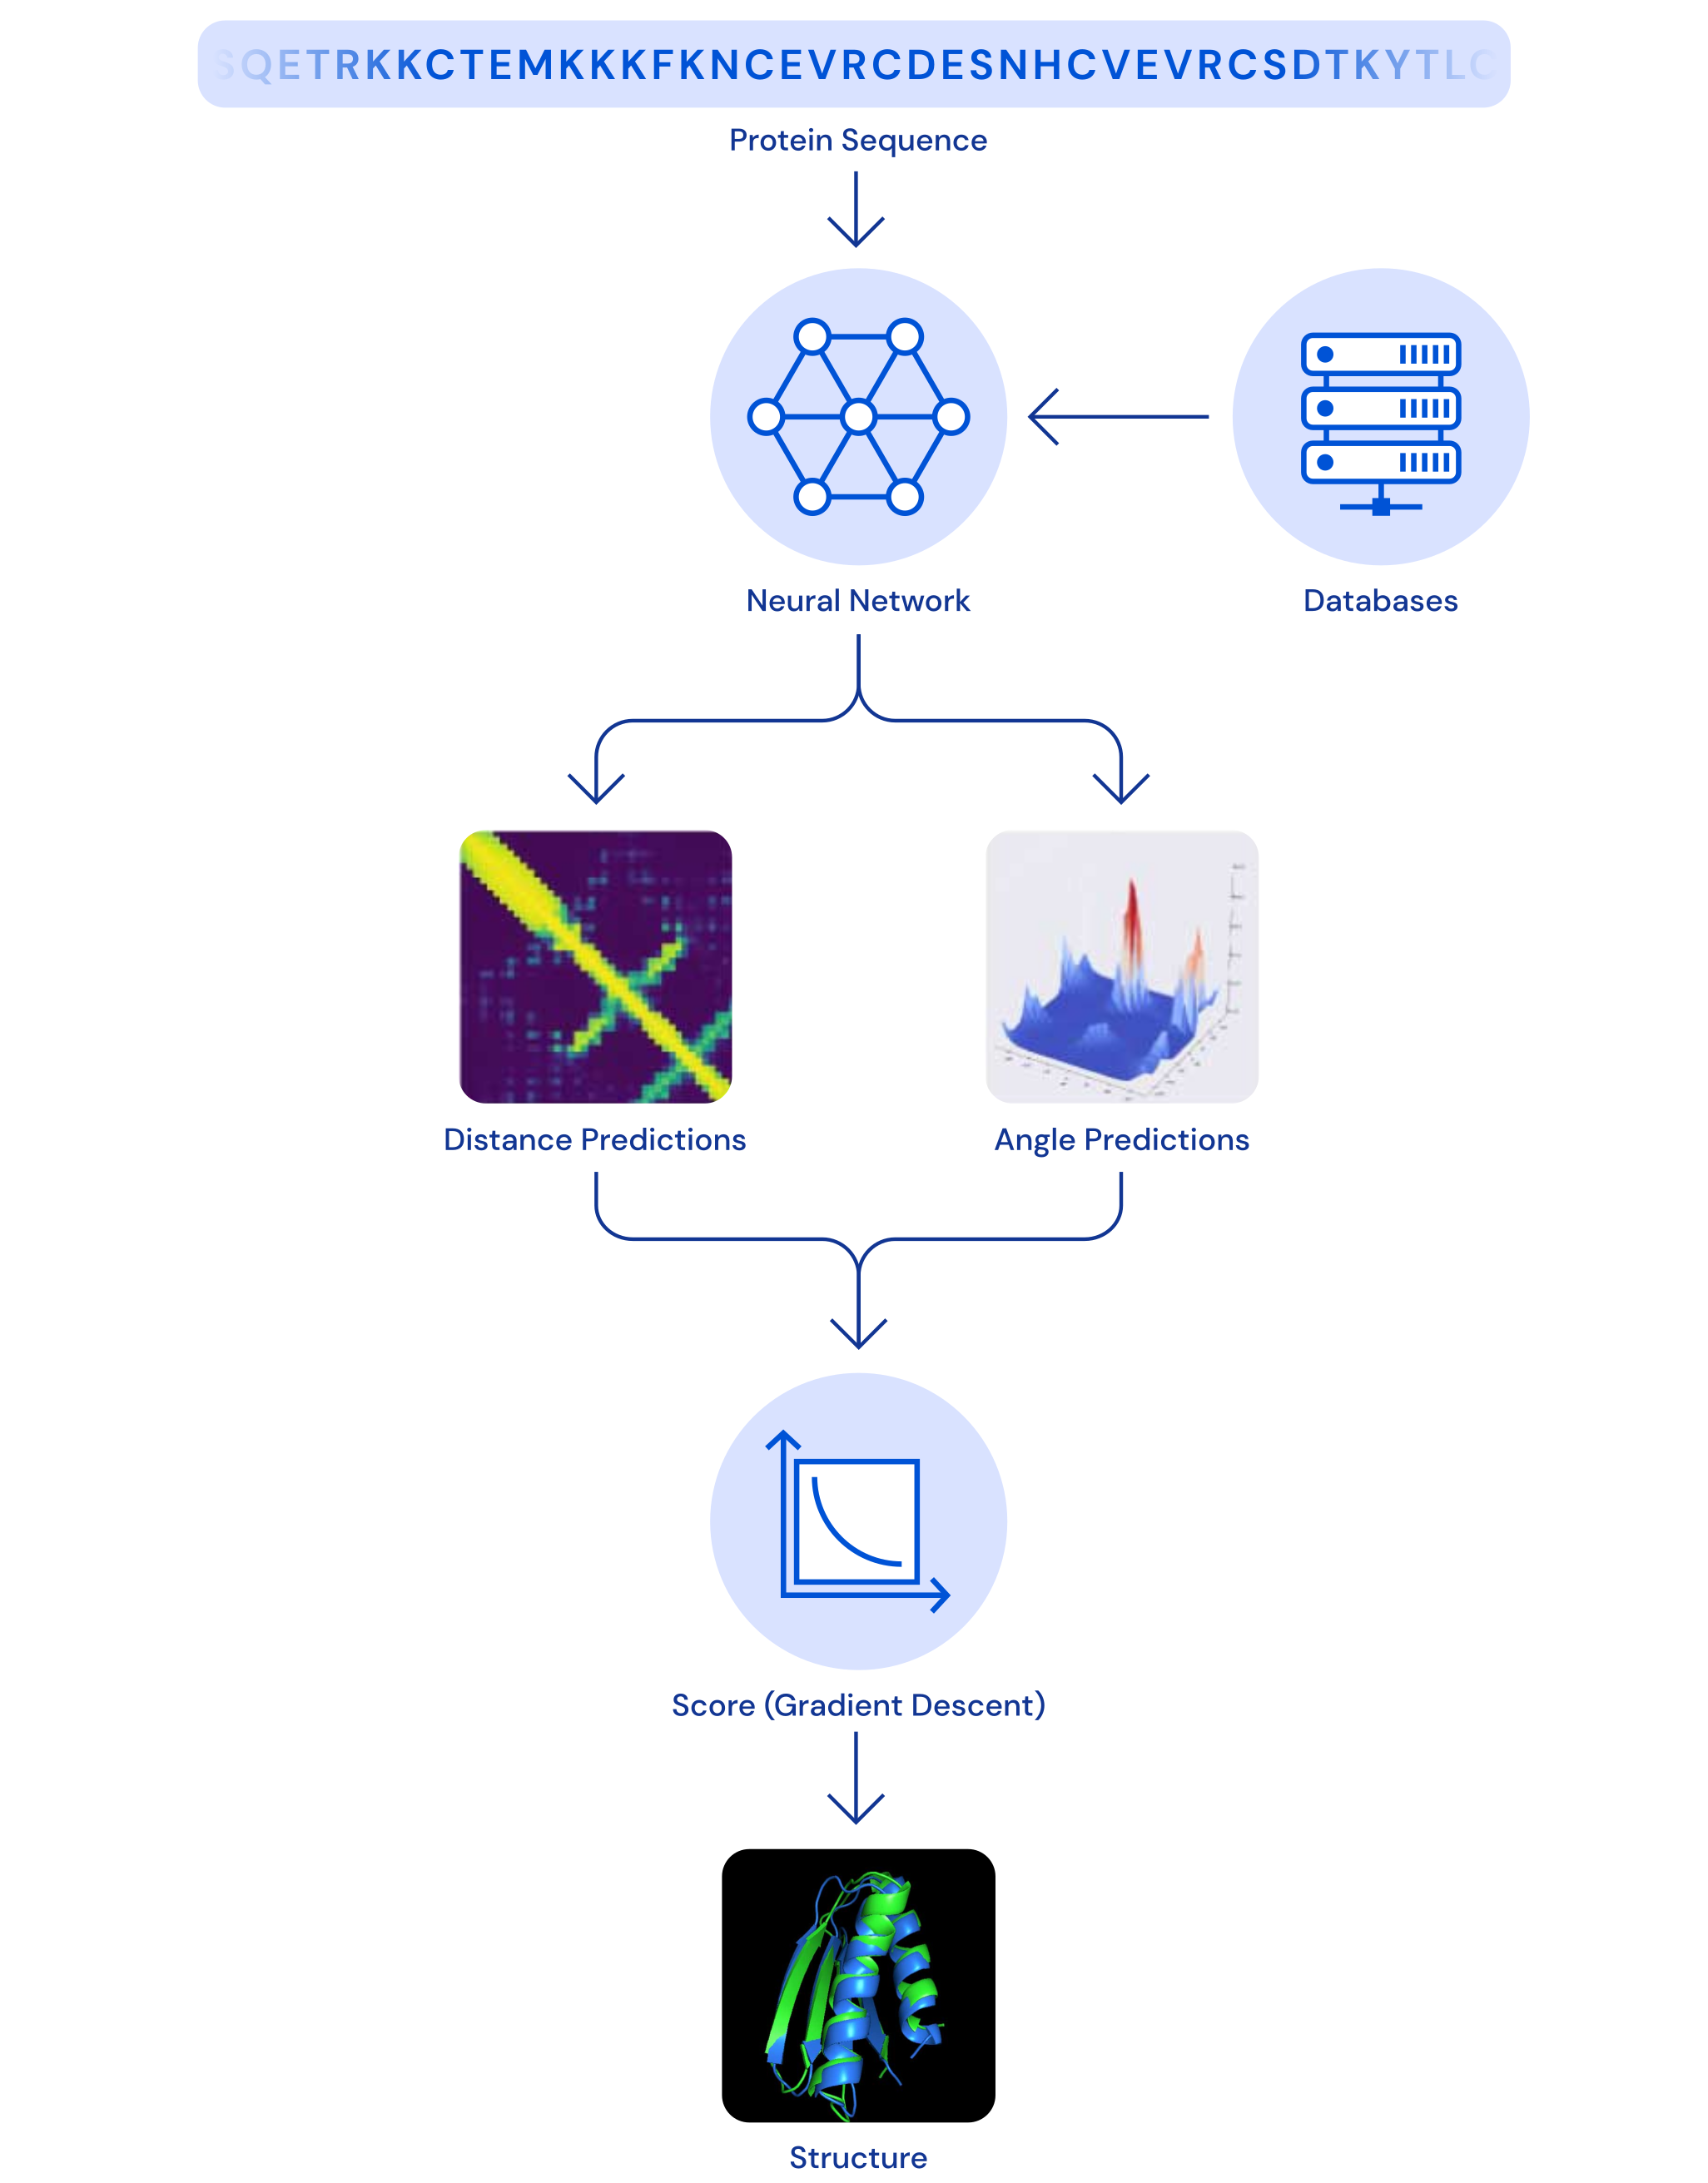
\includegraphics[width=0.45\textwidth]{AlphaFold-Blog-9c_diagram2.png}
        \caption*{{\footnotesize \textit {Diagram of Alpha Fold (source: Deepmind)}}}
        \rref[Senior et al. 2020]
    \end{figure}
\end{frame}

\begin{frame}{AI Art?}
    \begin{figure}
        \centering
        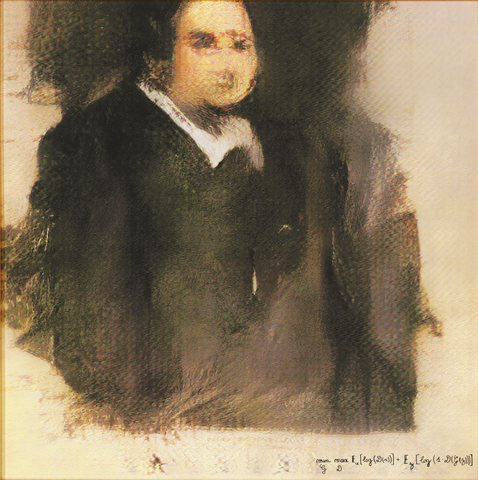
\includegraphics[width=0.5\textwidth]{478px-Edmond_de_Belamy.png}
        \caption*{\textit{Edmond de Bellamy} by Obvious(collective)}
    \end{figure}
    Generated using a Generative Adversarial Network.\\
    Selling prince (Oct. 2018): \$432,000
\end{frame}


%%%%%%%%%%%%%%%%%%%%%%%%
\begin{frame}[t]{Reasons for these recent achievements?}
    \begin{itemize}
        \item Increasing of the datasets in size and quality
        \only<1> {
        \begin{figure}
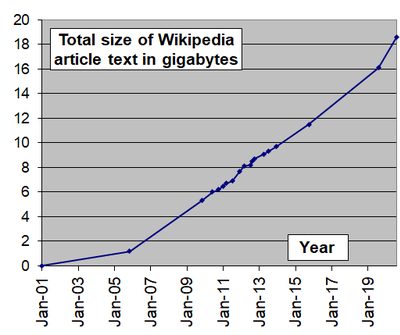
\includegraphics[width=.6\textwidth]{Wikipedia_article_size_in_gigabytes.png}
\end{figure}
\rref[source: Wikipedia]
}
        \item <2-> Progress in computing resources.
        \only<2> {
        \begin{figure}
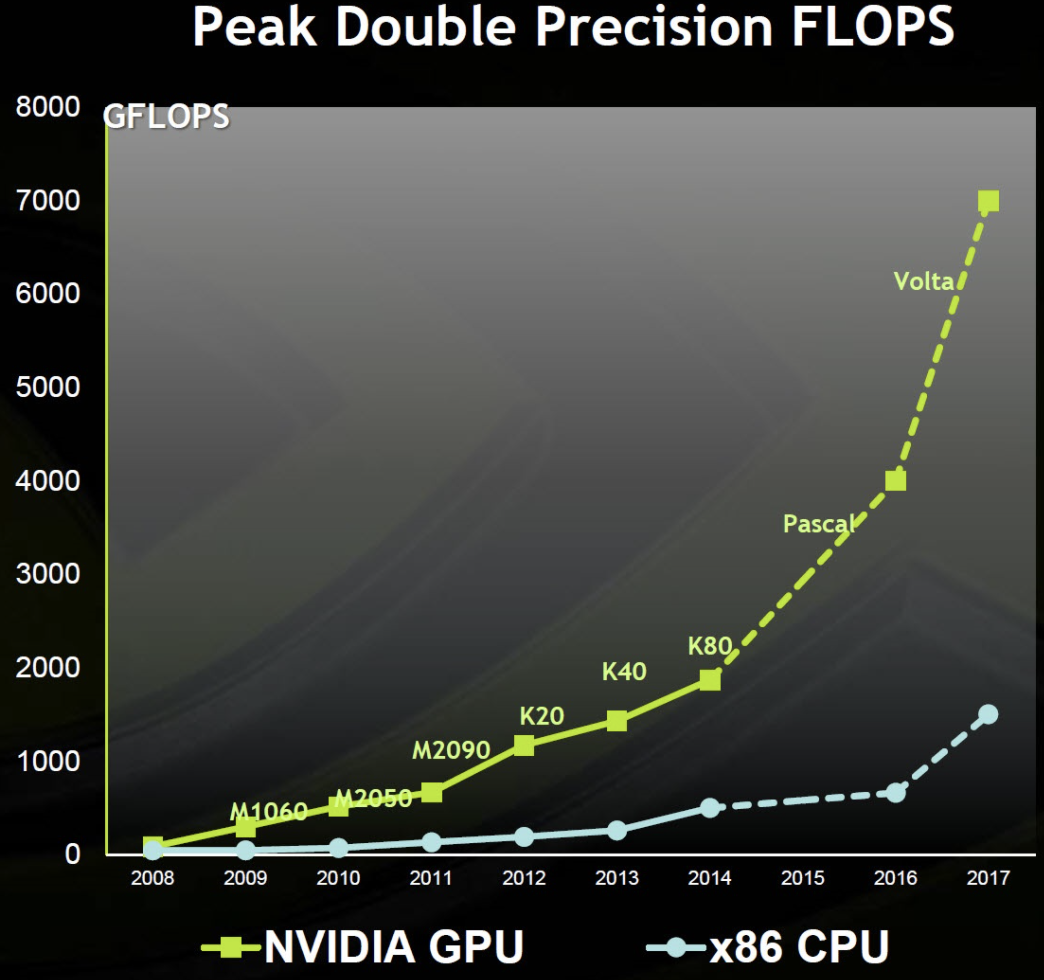
\includegraphics[width=.6\textwidth]{evolution-gpu.png}
\end{figure}
\rref[source: NVDIA]
}        
        
        \item <3-> Scientific research on new algorithms (e.g adapted to image processing)
                \only<3> {
        \begin{figure}
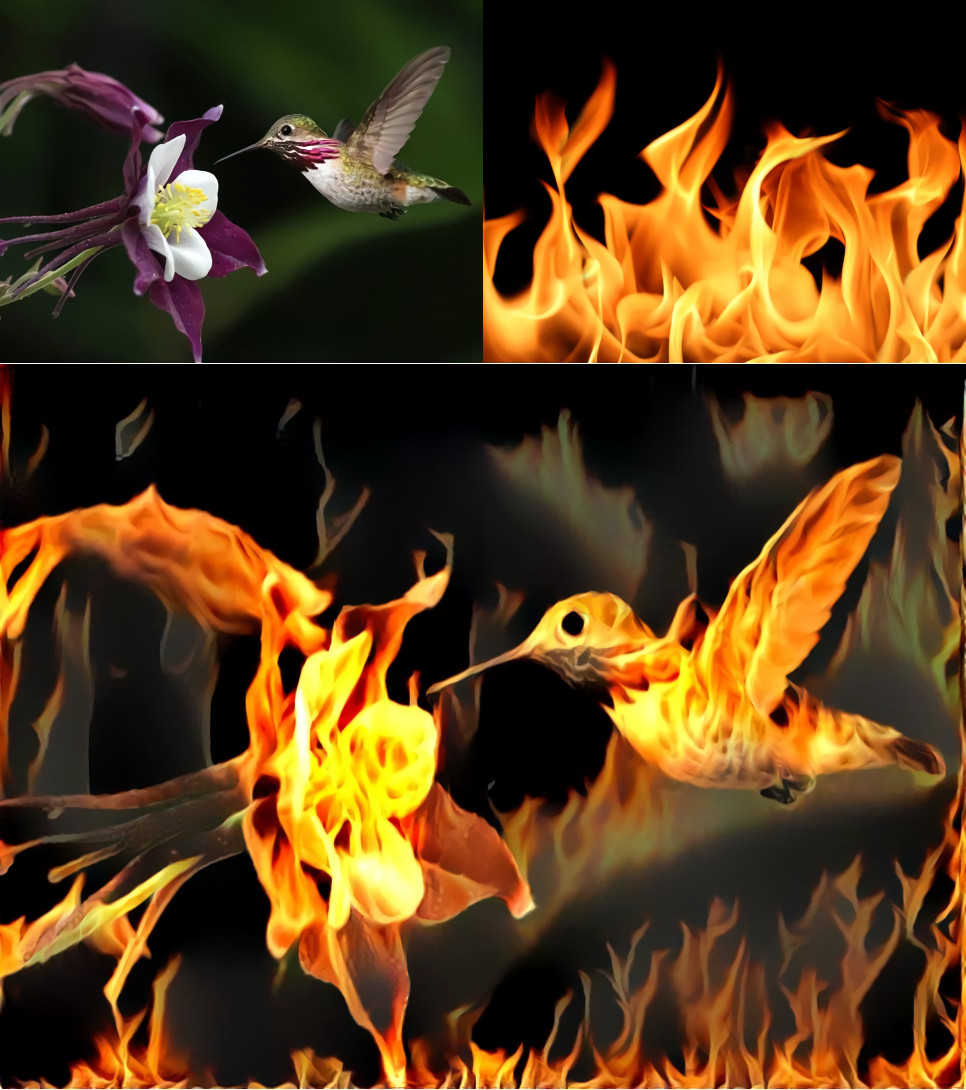
\includegraphics[width=.4\textwidth]{deep-art.jpg}
\end{figure}
\rref[source: Deep Dream Generator]

}      

\item<4-> Very efficient software (GPU, cloud computing, automatic differentiation, ...)
\only<4> {
\begin{center}
    \begin{tabular}{ccc}
        
\includegraphics[width=.25\textwidth]{TensorFlowLogo.png} &  
         
\includegraphics[width=.25\textwidth]{keraslogo.png}& 
         
\includegraphics[width=.25\textwidth]{pytorchlogo.png}\\
    \end{tabular}
\end{center}
}


\item<5-> Free software and open data culture.
\only<5> {
\begin{center}
    \begin{tabular}{cc}
        
\includegraphics[width=.25\textwidth]{ArXiv_logo.png} &  
         
\includegraphics[width=.25\textwidth]{GitHub-Logo.png}\\
    \end{tabular}
\end{center}
}

    \end{itemize}

\end{frame}

\begin{frame}{Apply Machine-Learning to physical (Earth-system) modelling?}
\alert{Why is it a good idea?}
    \begin{itemize}
        \item A increasing number of geophysical data (one spatial mission: 24 TB/day)
          \only<1> {
        \begin{figure}
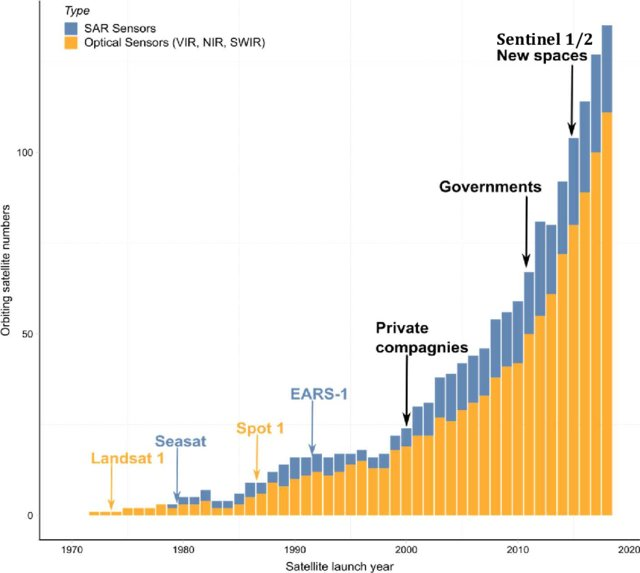
\includegraphics[width=.5\textwidth]{sat-eso.jpeg}
\caption*{Earth System observavtion satellites}
\end{figure}
\rref[source: Tonneau et al. (2020)]
}
        \item <2->Data with highly significant spatial patterns
                  \only<2> {
        \begin{figure}
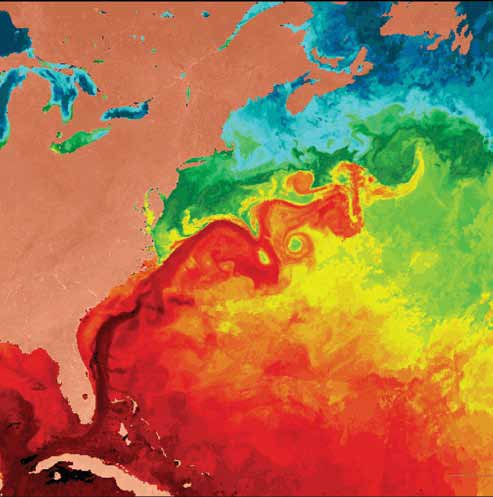
\includegraphics[width=.36\textwidth]{Satellite-image-of-sea-surface-temperature-showing-the-gulf-Stream-and-large-rings-and_W640.jpg}
\caption*{Sea Surface temperature of the gulf stream}
\end{figure}
\rref[source: Talley (2000)]
}
    \end{itemize}
\end{frame}

\begin{frame}{Why is physical modelling specific?}

\begin{columns}


\column{.5\textwidth}
\begin{figure}
    \caption*{NASDAQ Composite sock market index over the last 10 years}
    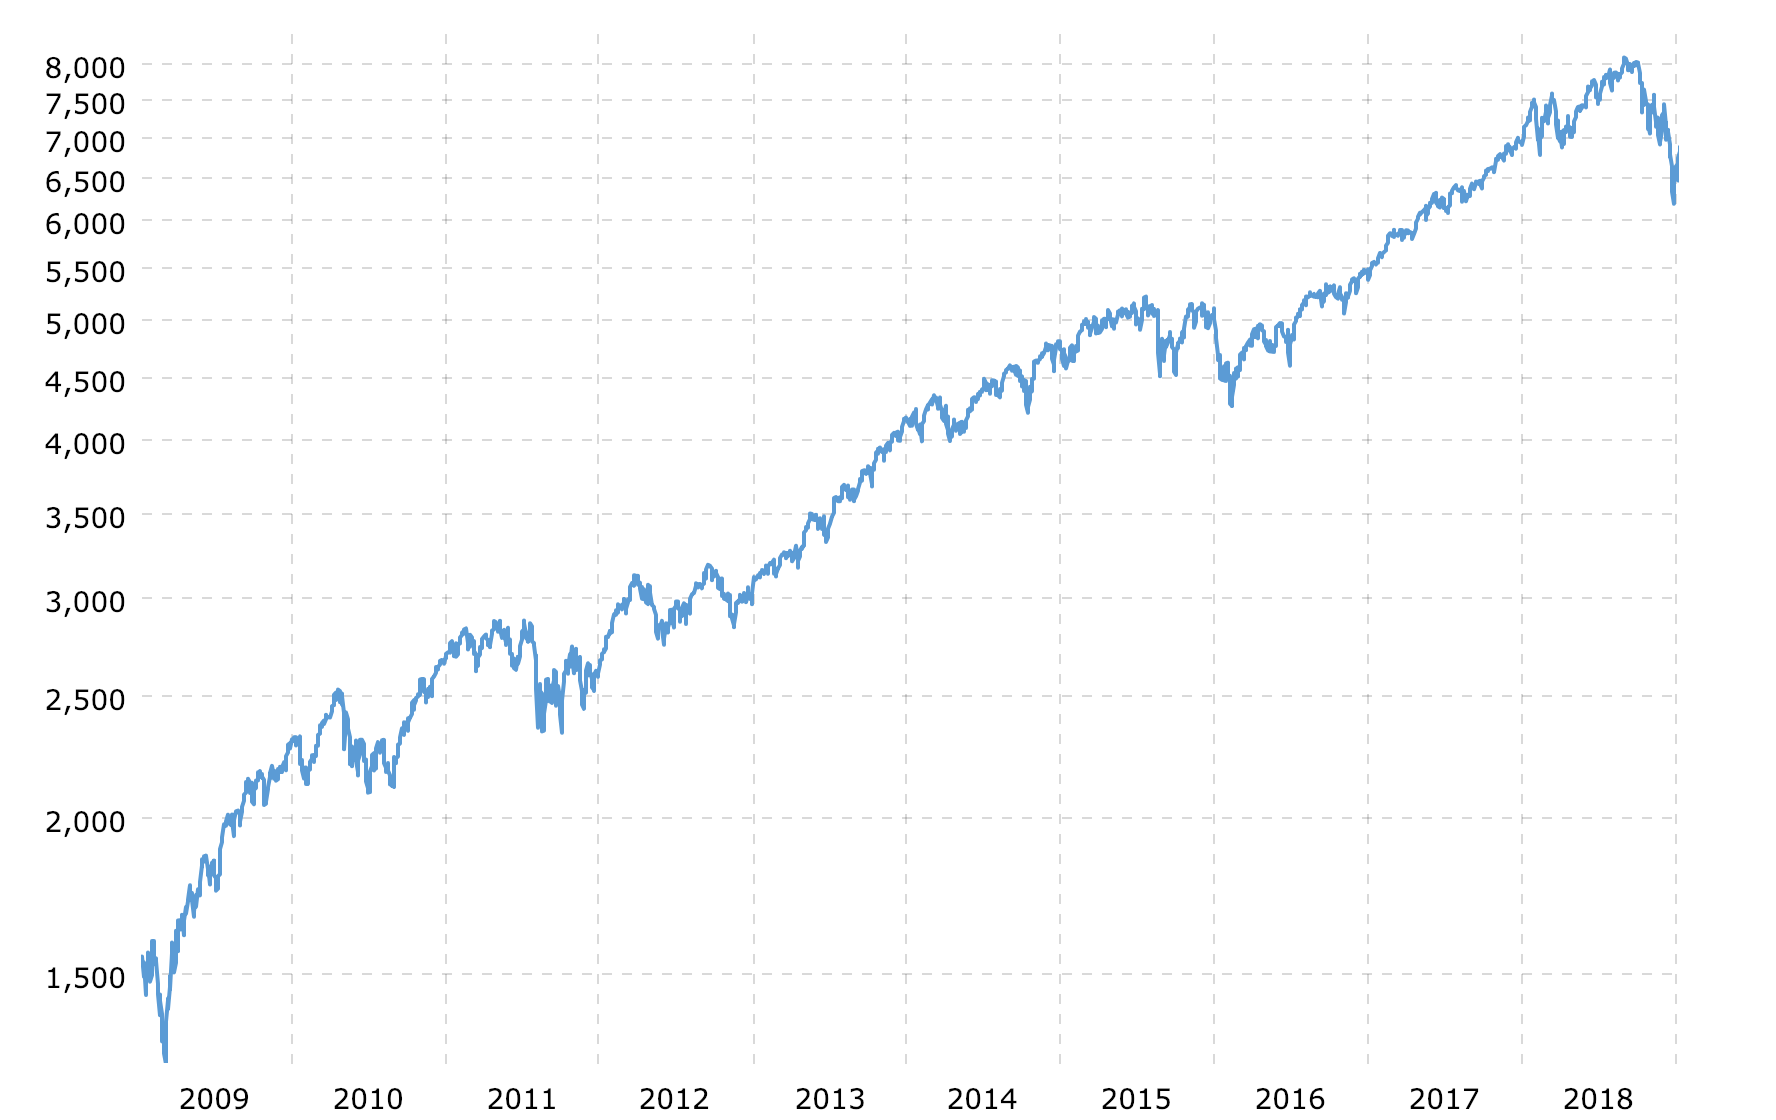
\includegraphics[width=\textwidth]{nasdaq-composite-index-10-year-daily-chart-2019-01-09-macrotrends.png}
\end{figure}
\visible<2->{\alert{Mostly unknown dynamical processes}}

\column{.5\textwidth}
\begin{figure}
\caption{IPCC, AR6, WG1}

    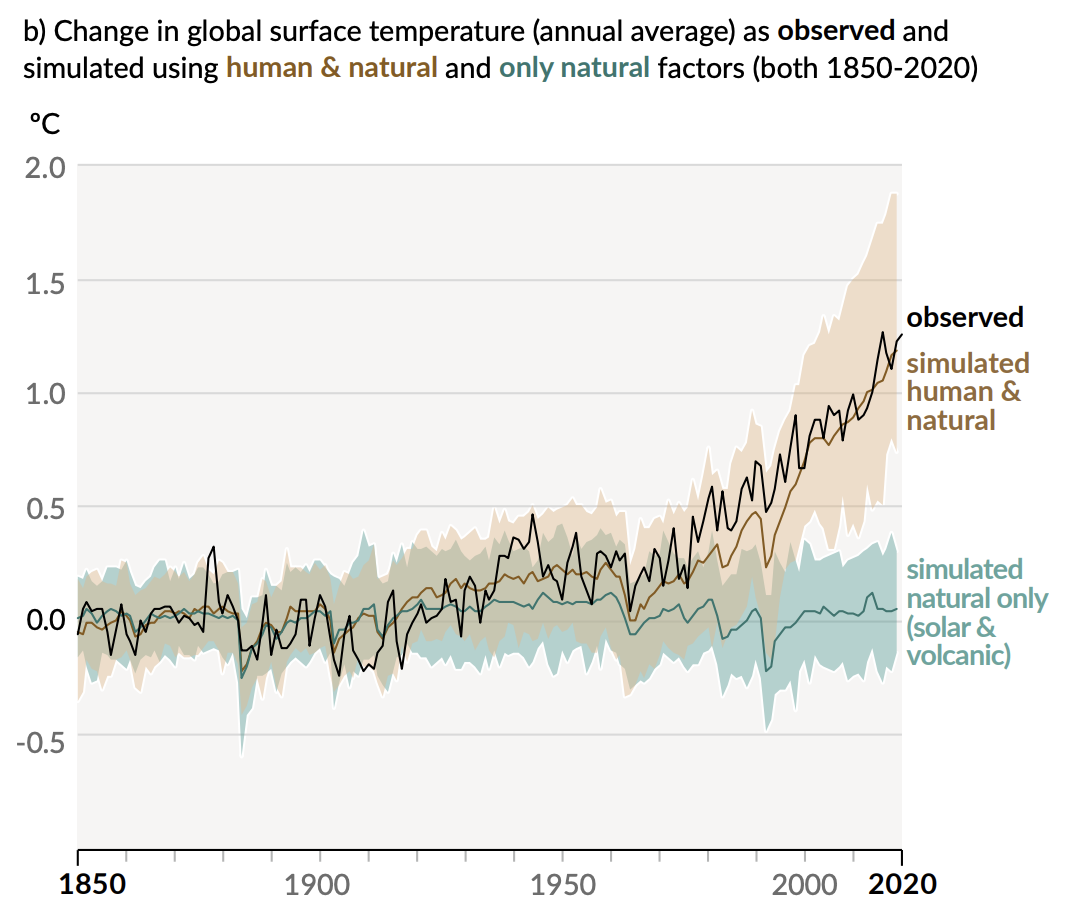
\includegraphics[width=\textwidth]{IPPC_temp.png}
\end{figure}
\visible<2->{\alert{Mostly known dynamical processes (based on physical principles)}}

\end{columns}
    
\end{frame}

\begin{frame}{What about data assimilation?}
    \alert{Machine learning and data assimilation are closely linked.}\\
 { \footnotesize   
     Some references:
 \begin{itemize}
     \item Geer, A.J., 2021. Learning earth system models from observations: machine learning or data assimilation?. {\it Philosophical Transactions of the Royal Society A}, 379(2194)
     \item  Brajard  et al. 2019. Connections between data assimilation and machine learning to emulate a numerical model. {\it Proceedings of the 9th International Workshop on Climate informatics}
     \item Bocquet et al. 2019. Data assimilation as a learning tool to infer ordinary differential equation representations of dynamical models. {\it Nonlinear processes in geophysics.} 26(3).
     \item Abarbanel, H.D., Rozdeba, P.J. and Shirman, S., 2018. Machine learning: Deepest learning as statistical data assimilation problems. {\it Neural computation, 30(8)}.
 \end{itemize}

}

\end{frame}

\section{Generalities on Machine Learning}
%%%%%%%%%%%%%%%%%%%%%
\begin{frame}
\frametitle{What is this about ?}
\begin{alertblock}{Can we extract knowledge, make some predictions, determine a "model" using this large
amount of data ?}

\end{alertblock}
\pause
\begin{figure}
\begin{tikzpicture} [
	auto,
	node distance = 1cm]
	\node(H0) [anchor=east]{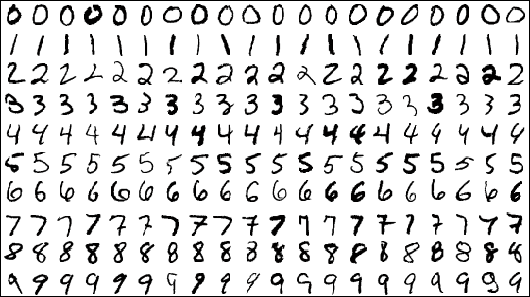
\includegraphics[width=0.4\textwidth]{mnistExamples.png}};
	\node(H1) [right of =  H0, xshift = .4\textwidth]  
	{Digit \newline $\in \{0,\ldots,9\}$};
	\node(legend) [below of = H0,yshift=-4ex]{Base of images};
	\draw [very thick, ->] (H0)--(H1);
\end{tikzpicture}
\end{figure}
\pause
\begin{itemize}
\item From high dimensional data (thousands to millions dimensions) to reduced dimensional data (less than 100)
\item From disorganized data to comprehensive information
\item \alert{Can we teach a machine how to do that ?}
\end{itemize}

\end{frame}

%%%%%%%%%%%%%%%%%%%%%%%%%
\begin{frame}
\frametitle{Two classes of Machine Learning problems}
\begin{enumerate}
\item \alert{Regression}: Determination of a quantitative variable from a set of data
\begin{itemize}
\item The price of a building from various predictors (Surface, ...)
\item A physical value (Temperature, humidity, ...) in the future knowing the past
\item ...
\end{itemize}
\pause
\item \alert{Classification}: Determination of a class 
\begin{itemize}
\item A digit from a image
\item Identification of the content of an image
\item ...
\end{itemize}
\end{enumerate}
\end{frame}
%%%%%%%%%%%%%%%%%%%%%%%%%%%
\begin{frame}
\frametitle{Two types of objectives}

\begin{enumerate}[<+->]
\item \alert{Supervised learning}: we have a set of labeled data with examples of targets.
\item \alert{Unsupervised learning}: we only have unlabeled the data, we have no examples of
what we want to obtain. We want to extract a "useful" representation of these data, or
some coherent categories.
\begin{itemize}
\item Determine typical behaviors of clients in a supermarket knowing what the have bought.
\end{itemize}
\item \alert{Semi-Supervised Learning}: Only a few subset of the data are labeled
\item \alert{Reinforcement Learning}: We can initiate and observe the interaction of an agent with its environment. We want to optimize the behavior of the agent.
\begin{itemize}
\item Playing a chess game.
\end{itemize}
\end{enumerate}
\end{frame}

%%%%%%%%%%%%%%%%%%%%
\begin{frame}
\frametitle{Formally}
\begin{block}{A Machine}
\begin{equation*}
y = \mathcal{M}(x,\theta)
\end{equation*}
\begin{itemize}
\item $x$: input
\item $y$: output
\item $\mathcal{M}$: a model (named "machine")
\item $\theta$ : parameters of the model $\mathcal{M}$.
\end{itemize}
\end{block}
\alert{Machine learning} consists in optimizing $\theta$ using a set of data. 
This is the training process.
\end{frame}



%%%%%%%%%%%%%%%%%%%%
\begin{frame}
\frametitle{The Machine Learning recipe}
\begin{block}{A Machine}
\begin{equation*}
y = \mathcal{M}(x,\theta)
\end{equation*}
\end{block}
What are \alert{the ingredients}? 
\begin{columns}[t]

\column{.6\textwidth}

\begin{itemize}
    \item<2-> Some \alert{data}
    \begin{itemize}
        \item $x,y$ : supervised learning
        \item only $x$: unsupervised learning
        \item $x$ and some subset of $y$: semi-supervised learning
    \end{itemize}
    
    
    \item<3-> An \alert{objective}
        \begin{itemize}
\item $y$ is quantitative: regression
\item $y$ is a class: classification
    \end{itemize}
    \end{itemize}
    
\column{.6\textwidth}

\begin{itemize}
    \item<4-> A computational architecture (the \alert{machine})
        \begin{itemize}
        \item linear
        \item non-linear
        \item neural networks, random forest, ...
    \end{itemize}
    \item<5-> A \alert{learning} process
    \begin{itemize}
        \item Estimation of $\theta$
    \end{itemize}
\end{itemize}

\end{columns}

\end{frame}
%%%%%%%%%%%%%%%%%%
\begin{frame}{Multidimensional data}
Generally, we have multidimensional data $X$ and a one-dimensional target $y$.
\begin{figure}
\begin{tikzpicture}
\draw [fill=blue!20](0,0) rectangle (2,3);
\draw [fill=blue!20](2.5,0) rectangle (3.5,3);

\node [text centered] at (1,3.3) {features};
\node[text centered, rotate=90] at (-0.3,1.5) {samples};
\node [text centered] at (1,1.5) {\Large $X$};
\node [text centered] at (3,1.5) {\Large $y$};

  %\draw [fill=blue:20,black] (0.,0.) rectangle (1,2) ; 
\end{tikzpicture}
 \end{figure}
\end{frame}

%%%%%%%%%%%%%%%%%%%%
\begin{frame}{An illustration}
\begin{columns}
\column{.6\textwidth}
\begin{itemize}
    \item Some \alert{Data}
    \begin{figure}
    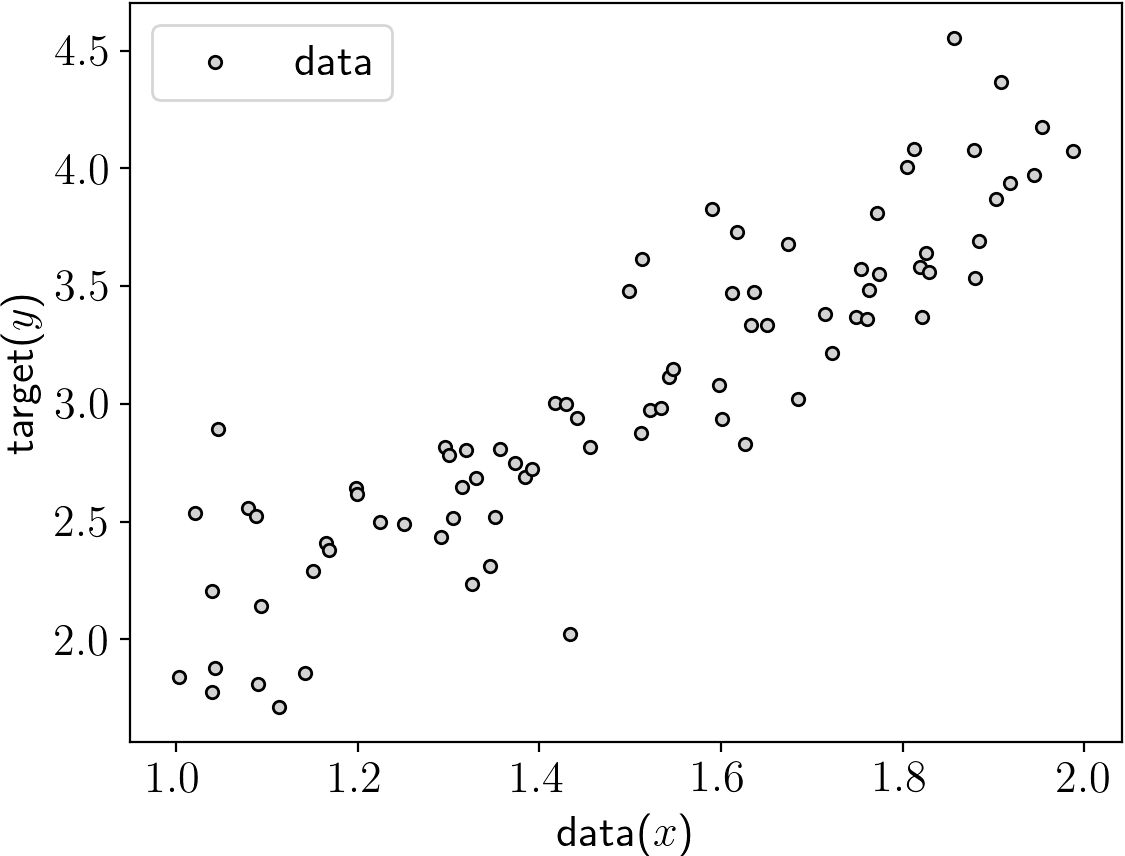
\includegraphics[width=.8\textwidth]{data-lin.png}
    \end{figure}

    \begin{itemize}
    \item there are labeled $y$: supervised learning
    \item $y$ is quantitative: regression
    \end{itemize}
\pause
\item An \alert{Objective}: Estimate $\hat{y}$ from $x$ by minimizing $(\hat{y}-{y})^2$ (Least-square objective)

\end{itemize}
\column{.5\textwidth}
\begin{itemize}
\pause
    \item A \alert{model}: $\hat{y} = \theta_1 X + \theta_0$ (linear)
\pause
    \item A \alert{learning} process:
    $\mathbf{\theta}=(\mathbf{X}^T\mathbf{X})^{-1}\mathbf{X}^Ty$
\end{itemize}
\pause
\begin{block}{Result}
    \begin{figure}
    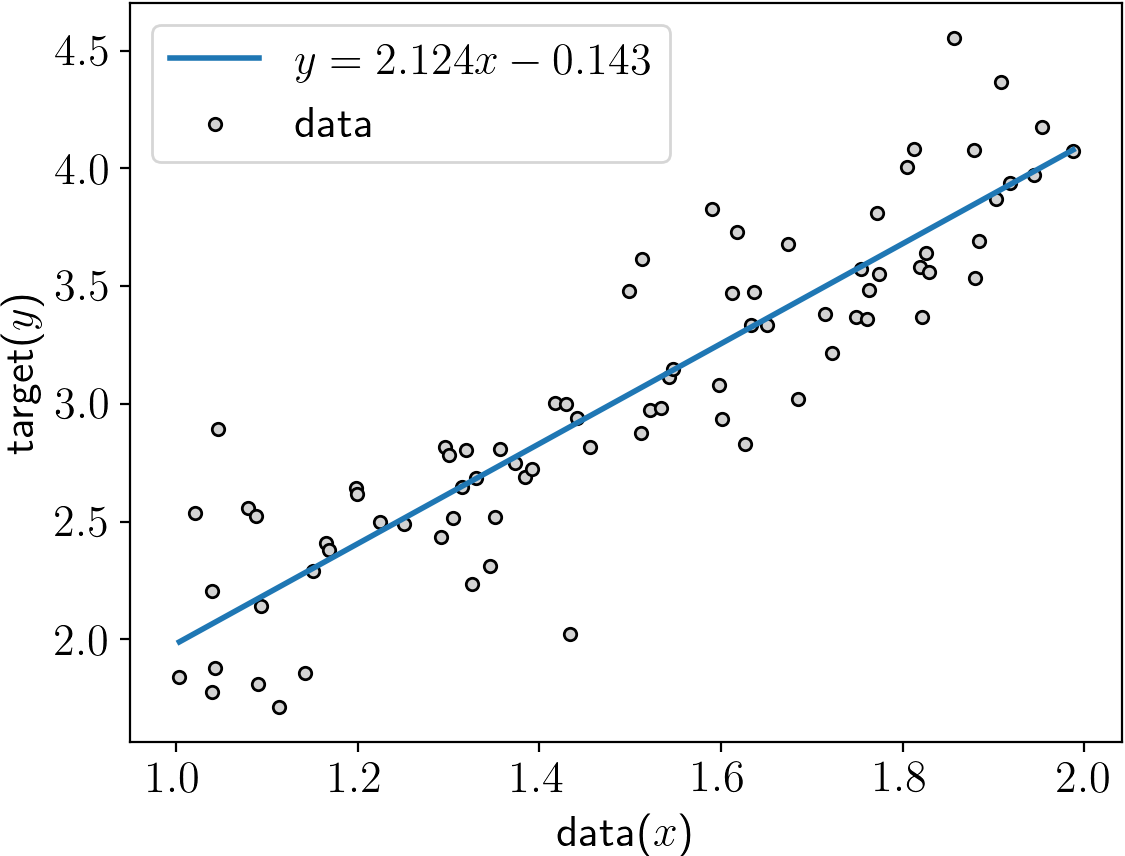
\includegraphics[width=.9\textwidth]{interp-lin.png}
    \end{figure}
\end{block}
\end{columns}
\end{frame}




\end{document}